% Plantilla LLNCS para Springer Computer Science Proceedings
\documentclass[runningheads]{llncs}

\usepackage[T1]{fontenc}
\usepackage[utf8]{inputenc}
\usepackage{graphicx}
\usepackage{hyperref}
\usepackage{color}
\usepackage{textgreek}
\usepackage{amsmath}
\usepackage{float}
\renewcommand\UrlFont{\color{blue}\rmfamily}

% Parámetros de flotado más permisivos para empaquetar figuras/tablas y evitar huecos
\renewcommand{\topfraction}{0.92}
\renewcommand{\bottomfraction}{0.85}
\renewcommand{\textfraction}{0.06}
\renewcommand{\floatpagefraction}{0.75}
\setcounter{topnumber}{3}
\setcounter{bottomnumber}{2}
\setcounter{totalnumber}{5}

\begin{document}

\title{Semantic Search of Scientific Abstracts through HNSW
Indexing in Vector Databases}

\author{Santiago Callocondo-Garay\inst{1}\orcidID{0009-0007-2794-5097} \and
Piero Mejia-Ramos\inst{1}\orcidID{0009-0006-3011-0640} \and
Antonio Arroyo-Paz\inst{1}\orcidID{0000-0003-1838-4527}}

\authorrunning{S. Callocondo, P. Mejia and A. Arroyo}
\titlerunning{Semantic Search with HNSW in Scientific Abstracts}

\institute{Escuela Profesional de Ingeniería de Sistemas, Universidad Nacional de
San Agustín, Arequipa, Perú\\
\email{\{scallocondo,pmejia,aarroyop\}@unsa.edu.pe}}

\maketitle

\begin{abstract}
Exact nearest-neighbor search stops being practical once a corpus reaches millions of
documents: the cost simply explodes. That is why large-scale semantic retrieval leans
on approximate nearest-neighbor (ANN) search. The most popular of these algorithms
today is Hierarchical Navigable Small World (HNSW), yet little is known about how it
fares on scientific abstracts ---a domain with a sprawling range of topics and a
dense, specialized vocabulary. We put it to the test on FAISS, over a collection of
49,000 arXiv abstracts. We compare two very different embedding models, SciBERT
(specialized in scientific language) and E5-large (general purpose), across 36
configurations that mix the number of connections per node ($M$), the construction
breadth (\textit{ef\_construction}), and the similarity metric (cosine and L2); each
one is measured against an exact brute-force search using Recall@K, MRR, and latency.
$M$ is the factor that matters: raising it from 8 to 16 lifts Recall@10 from roughly
0.95 to above 0.98, whereas \textit{ef\_construction} barely adds accuracy and nearly
triples build time. The best configuration ---SciBERT with cosine, $M=32$, and
\textit{ef\_construction}$=400$--- reaches a Recall@10 of 0.998 and an MRR of 1.000,
answering each query in 0.33\,ms. Despite its lower dimensionality, SciBERT runs
faster and slightly leads on this fidelity metric. That ranking reverses, however, on
realistic short natural-language queries: there E5-large clearly wins (Recall@10 of
0.95 versus 0.19 for SciBERT), making it the model to deploy in a real search engine.
We also release an interactive demo that turns the configuration into a working search
engine over the indexed corpus.

\keywords{HNSW \and semantic search \and scientific embeddings \and FAISS \and
Recall@K}
\end{abstract}

\section{Introduction}
% -------------------------------------------------------

% Paragraph 1 — Conceptual Framework: The Problem and Its Significance
The volume of scientific literature is growing faster than any conventional
search technique can keep up with. This is evident in the figures: as of May 2026,
arXiv contained more than 2.6 million publications \cite{ref1}, while PubMed
indexed more than 38 million biomedical records \cite{ref2}. Since two
abstracts can convey the same idea without using the same phrase, searching for
keyword matches in collections such as these is ineffective. To bridge
this gap, existing algorithms capture semantic similarity beyond
literal vocabulary by representing each document as a high-dimensional dense
vector, or \textit{embedding} \cite{ref3}. However, when performing queries, the problem
resurfaces. Retrieving the exact nearest neighbor requires comparing the
query against all vectors in the corpus: an $O(N \cdot d)$ cost that grows
linearly with the collection and, over millions of documents, makes latency
unfeasible. Therefore, large-scale access relies on finding the nearest neighbors, which sacrifices some precision for a fast response \cite{ref4}.

Among artificial neural network algorithms, the Hierarchical Navigable Small World (HNSW) algorithm \cite{ref5} has become the standard algorithm for large-scale semantic search. It is based on the concept of small-world network theory \cite{ref6}: it organizes vectors into a multilayer hierarchical structure to resolve each query with a time complexity of $O(\log N)$ and achieves a recall rate of over 97\% in performance tests \cite{ref5}. It is no coincidence that it has become the primary index for platforms such as FAISS \cite{ref7} and Milvus \cite{ref8}. However, this performance is not static. On the one hand, it depends on the index parameterization: the tuning of $M$ and \texttt{ef\_construction} determines the balance between construction cost and recall quality \cite{ref9}.

This depends on similarity measures, whose effects have been studied primarily in the context of retrieval-augmented generation (RAG) \cite{ref10}; Elkiran and Rasheed \cite{ref11} compared cosine distance, scalar product distance, and Euclidean distance on the SQuAD corpus \cite{ref12}. Unfortunately, all of this data comes from general corpora rather than specialized scientific terminology.

% Paragraph 3 — Knowledge Gap
The HNSW model has been extensively studied, but it has encountered difficulties with scientific summaries, where terminology is domain-specific and topics are unevenly distributed. We needed a test domain to compare different models—for example, domain-specific models such as SciBERT and general models such as E5-large—and to thoroughly evaluate the influence of $M$, \texttt{ef\_construction}, and similarity factors on $K$ and $MRR$ performance. As long as this shortcoming persists, currently accepted parameterization recommendations cannot be directly applied to practical studies in the scientific literature.

The objective of this work is to evaluate the performance of the FAISS-indexed HNSW database in abstract semantic search on arXiv and to compare SciBERT with E5-large for $M$, $\texttt{ef\_construction}$, and different combinations of similarity features. In particular, we seek a parameterization scheme that minimizes overestimation and maximizes Recall@$K$ and $MRR$ in scientific literature searches. We also evaluate whether a model's advantage holds when the query is a short natural-language phrase—as is typical in real-world use of the system—rather than a full abstract.

% -------------------------------------------------------
\section{Related Work}
% -------------------------------------------------------

The emergence of artificial neural network (ANN) algorithms offers a practical solution to the problem of the excessive computational cost of exact $k$-nearest-neighbor algorithms in high-dimensional spaces. Mathur and Chhabra \cite{ref4} classified them into four categories: exhaustive search, trees, quantization, and graph-based methods. They observed that graph-based methods perform better as the scale increases. HNSW \cite{ref5} falls into this category: inspired by small-world networks \cite{ref6}, it creates a multilayer hierarchical structure where the upper layer provides numerous sparse hops and the lower layer optimizes the local search with a query cost of $O(\log N)$. Many optimization techniques have been developed based on this basic idea. Iwasaki and Miyazaki \cite{ref13} accelerated queries on large-scale data by adjusting the input and output rates of each node (removing unnecessary edges without loss of precision).


Zhao et al. \cite{ref14} criticized the development cost of LSH-APG, a lightweight search method based on a locality-based hashing algorithm that allows for point insertion and maintains an incremental graph as the cluster grows.


The true weakness of HNSW lies not in the query itself, but in the representation. Each insertion results in multiple multi-layer passes and a series of distance calculations [9]. Feifang Zhao et al. [9] propose H-DMax, which includes the parameter λ to hierarchically prune the most distant neighbors. This pruning is abrupt in the lower layers and gradual in the upper layers to maintain overall connectivity. This enables representation speedups of up to 1.27x compared to SIFT1M (λ = 1.10), while the recall loss is less than 0.27. Product quantization [15] takes a different approach: it compresses vectors into short codes and offers the greatest assembly acceleration (3.6x) compared to FAISS [7]. However, this method comes at a high cost: recall can drop to as low as 85\%, and it cannot be used when accuracy must be guaranteed.

In terms of infrastructure, FAISS \cite{ref7} and Milvus \cite{ref8} have set the standard for implementing HNSW metrics in production environments. Milvus supports cosine, dot product, and $L_2$ normalization on dense and mixed embeddings and forms the basis of many state-of-the-art RAG pipelines \cite{ref10}. On this platform, Elkiran and Rasheed \cite{ref11} tested three metrics using OpenAI embeddings (3,072 dimensions) and the SQuAD corpus \cite{ref12}: cosine and dot product achieved $\text{R}@10 = 0.909$--$0.925$ and $\text{MRR} = 0.781$--$0.793$, respectively, while the unnormalized $\text{LRR}$ was $0.116$. As indicated in the classical theory of information retrieval \cite{ref16}, the similarity threshold determines the trade-off between precision and recall, and normalization is crucial when using $L_2$.

A review of the literature revealed significant gaps. To date, no 
study has evaluated the HNSW algorithm using dense and 
irregularly distributed scientific abstracts. Furthermore, there is no framework for comparing scientific 
embedding models (such as SciBERT and E5-large) when evaluating the 
performance of $M$ and \textit{ef\_construction} with respect to $\text{Recall}@K$ and $\text{MRR}$. 
Due to a lack of understanding of the semantic properties of 
academic texts, research in RAG remains limited to the use of common datasets 
for the question-answering task \cite{ref11,ref12}.

% -------------------------------------------------------
\section{Methodology}
% -------------------------------------------------------

% -------------------------------------------------------
\subsection{Dataset}
% -------------------------------------------------------

We worked with arXiv-abstracts-2021 (CC0 license), an open-access collection of approximately two million abstracts uploaded to arXiv \cite{ref17}. Since the dataset was too large for a reasonable experimental budget, we reduced its size. From these two million abstracts, we extracted $50\,000$ using stratified sampling by category. Why did we choose stratified sampling over random sampling? Because arXiv does not distribute its papers uniformly: for example, physics is much more heavily represented than quantitative biology. Simple random sampling would concentrate the papers in a few dominant areas and eliminate precisely what we wanted to investigate, namely, the thematic heterogeneity in scientific language. Stratified sampling preserves this diversity in physics, mathematics, computer science, and biology in proportions similar to those of the original dataset.

We recorded three fields from each record: \texttt{descriptor}, \texttt{abstract}, and \texttt{category}. Other metadata—author, DOI, and journal references—were excluded since they did not contribute to semantic searches.

% -------------------------------------------------------
\subsection{Embedding Models}
% -------------------------------------------------------

We compared two contrasting representations of ideas. SciBERT \cite{ref18} produces 768-dimensional vectors and is naturally trained on scientific literature; therefore, it is already familiar with the vocabulary, abbreviations, and expressions typical of technical abstracts. In contrast, E5-large \cite{ref19} produces 1024-dimensional vectors and comes from a broader field; its advantage lies not in its area of specialization, but in its size and relative ease of memorization during training.

The fundamental question is which carries more weight: mastery of scientific vocabulary or specific training for retrieval. SciBERT has a thorough understanding of technical jargon but was not trained to match queries with documents; E5-large was, even though it comes from a general domain. Which of these two properties is decisive is an empirical question, and this study answers it.

% -------------------------------------------------------
\subsection{Experimental Design}
% -------------------------------------------------------

We used FAISS \cite{ref7} for indexing. We ruled out ChromaDB because it adds a layer of abstraction without providing any experimental signal, whereas FAISS offers low-level access to the HNSW graph parameters—exactly what we needed to manipulate.

We varied three factors. The parameter $M$—the number of connections per node—takes values in $\{8, 16, 32\}$. The parameter \texttt{ef\_construction}—the scope of the search during index construction—takes values from $\{100, 200, 400\}$. The similarity metric varies between the cosine distance and the Euclidean distance ($L_2$). The query search depth (\texttt{ef\_search}) was set to 50 in all experiments. The combination of the two embedding models with these three axes yields 36 configurations, each indexed and evaluated separately (Table~\ref{tab:factores}).

\begin{table}[tbp]
\caption{Experimental design factors and their levels. The full combination
$2 \times 3 \times 3 \times 2$ yields 36 configurations.}\label{tab:factores}
\centering
\begin{tabular}{|l|l|c|}
\hline
\textbf{Factor} & \textbf{Levels} & \textbf{Count} \\
\hline
Embedding model & SciBERT (768d), E5-large (1024d) & 2 \\
Parameter $M$ & 8, 16, 32 & 3 \\
\textit{ef\_construction} & 100, 200, 400 & 3 \\
Similarity metric & Cosine, L2 & 2 \\
\hline
\multicolumn{2}{|r|}{\textbf{Total configurations}} & \textbf{36} \\
\hline
\end{tabular}
\end{table}

% -------------------------------------------------------
\subsection{Construction of the \textit{ground truth}}
% -------------------------------------------------------

To determine whether HNSW is accurate, we need a truth against which to compare it, and that
truth is the exact search. From the 50,000 abstracts, we set aside 1,000 as
queries—also using stratified sampling—and kept the remaining 49,000
as the indexed corpus. With this dataset, we create a simple index that covers the internal space and 
returns the nearest neighbors for each query. \textit{IndexFlatL2} uses the 
Euclidean distance metric, while \textit{IndexFlatIP} implements the 
inner product metric (associated with cosine similarity). This method is not scalable 
on its own; by definition, it produces exact results, but at a high computational cost. 
Each query is processed in two stages: the first run establishes the exact indexing 
and returns the $K$ actual neighbors (brute force). In the second run, the 
HNSW index is applied, and the approximate runtime is measured. Comparing 
both lists reveals the extent to which HNSW sacrifices accuracy in exchange for speed.

% -------------------------------------------------------
\subsection{Evaluation Metrics}
% -------------------------------------------------------

We measure three metrics. The first is $\text{Recall}@K$, which is defined as the fraction of the $K$ true neighbors 
that the HNSW algorithm is able to retrieve. We calculate the success rate for 
$K \in \{1, 5, 10\}$ and observe the performance for larger lists. Another 
quality metric used is the mean reciprocal rank ($\text{MRR}$), 
which evaluates the position of the first relevant result that appears at the 
top and penalizes those with a lower ranking. On the other hand, request latency 
(measured in milliseconds) represents the actual time cost to the user. 
At this point, it is important to clarify that these actual neighbors are not obtained 
from human correlation inferences, but rather through an exact brute-force search 
within the same vector space. Therefore, $\text{Recall}@K$ and $\text{MRR}$ 
measure the reliability of HNSW through the strict accuracy of the searches, 
rather than through correlations perceived by real users.

Consequently, \textit{Recall} and $\text{MRR}$ represent the system's quality, 
while latency represents speed. The importance of this study lies 
precisely in the trade-off between these parameters; since there is no 
universally perfect setting, our goal is to identify and analyze these 
trade-offs.

To determine whether the differences observed between SciBERT and E5-large are statistically significant given the variability across queries, we applied paired tests to the same set of 1,000 queries. We used the exact binomial version of the McNemar test on the binary accuracy of $\text{Recall}@10$ and the signed Wilcoxon rank-sum test on the per-query values of $\text{Recall}@10$ and the reciprocal rank. We report the two-sided $p$-value and the rank-biserial effect size, with a significance level of $\alpha = 0.05$.

Since the previous evaluation uses full abstracts as queries—which measures the accuracy of the index but not the actual use of the system, where the user formulates a short phrase in natural language—we supplement it with a \textit{known-item} evaluation. On a reproducible sample of 1,000 documents from the corpus, we use their title—a phrase of about ten words—as the query; the title is not part of the index, and the relevant document is unambiguous: the abstract from which it originates. The titles are vectorized using the same procedure as the corpus and are retrieved using the best configuration, measuring $\text{Recall}@K$ and the MRR for retrieving the original abstract.

% -------------------------------------------------------
\section{System Implementation}
% -------------------------------------------------------

The implemented system consists of a \textit{pipeline}
whose purpose is to systematically build, index, and evaluate the 36 configurations defined in Section 3. Its architecture consists of four linked stages: corpus ingestion and sampling, vectorization, indexing using HNSW, and evaluation. These stages must be deployed on a distributed computing infrastructure across two execution environments. Fig.~\ref{fig:diagrama} illustrates this organization.

\begin{figure}[t]
\centering
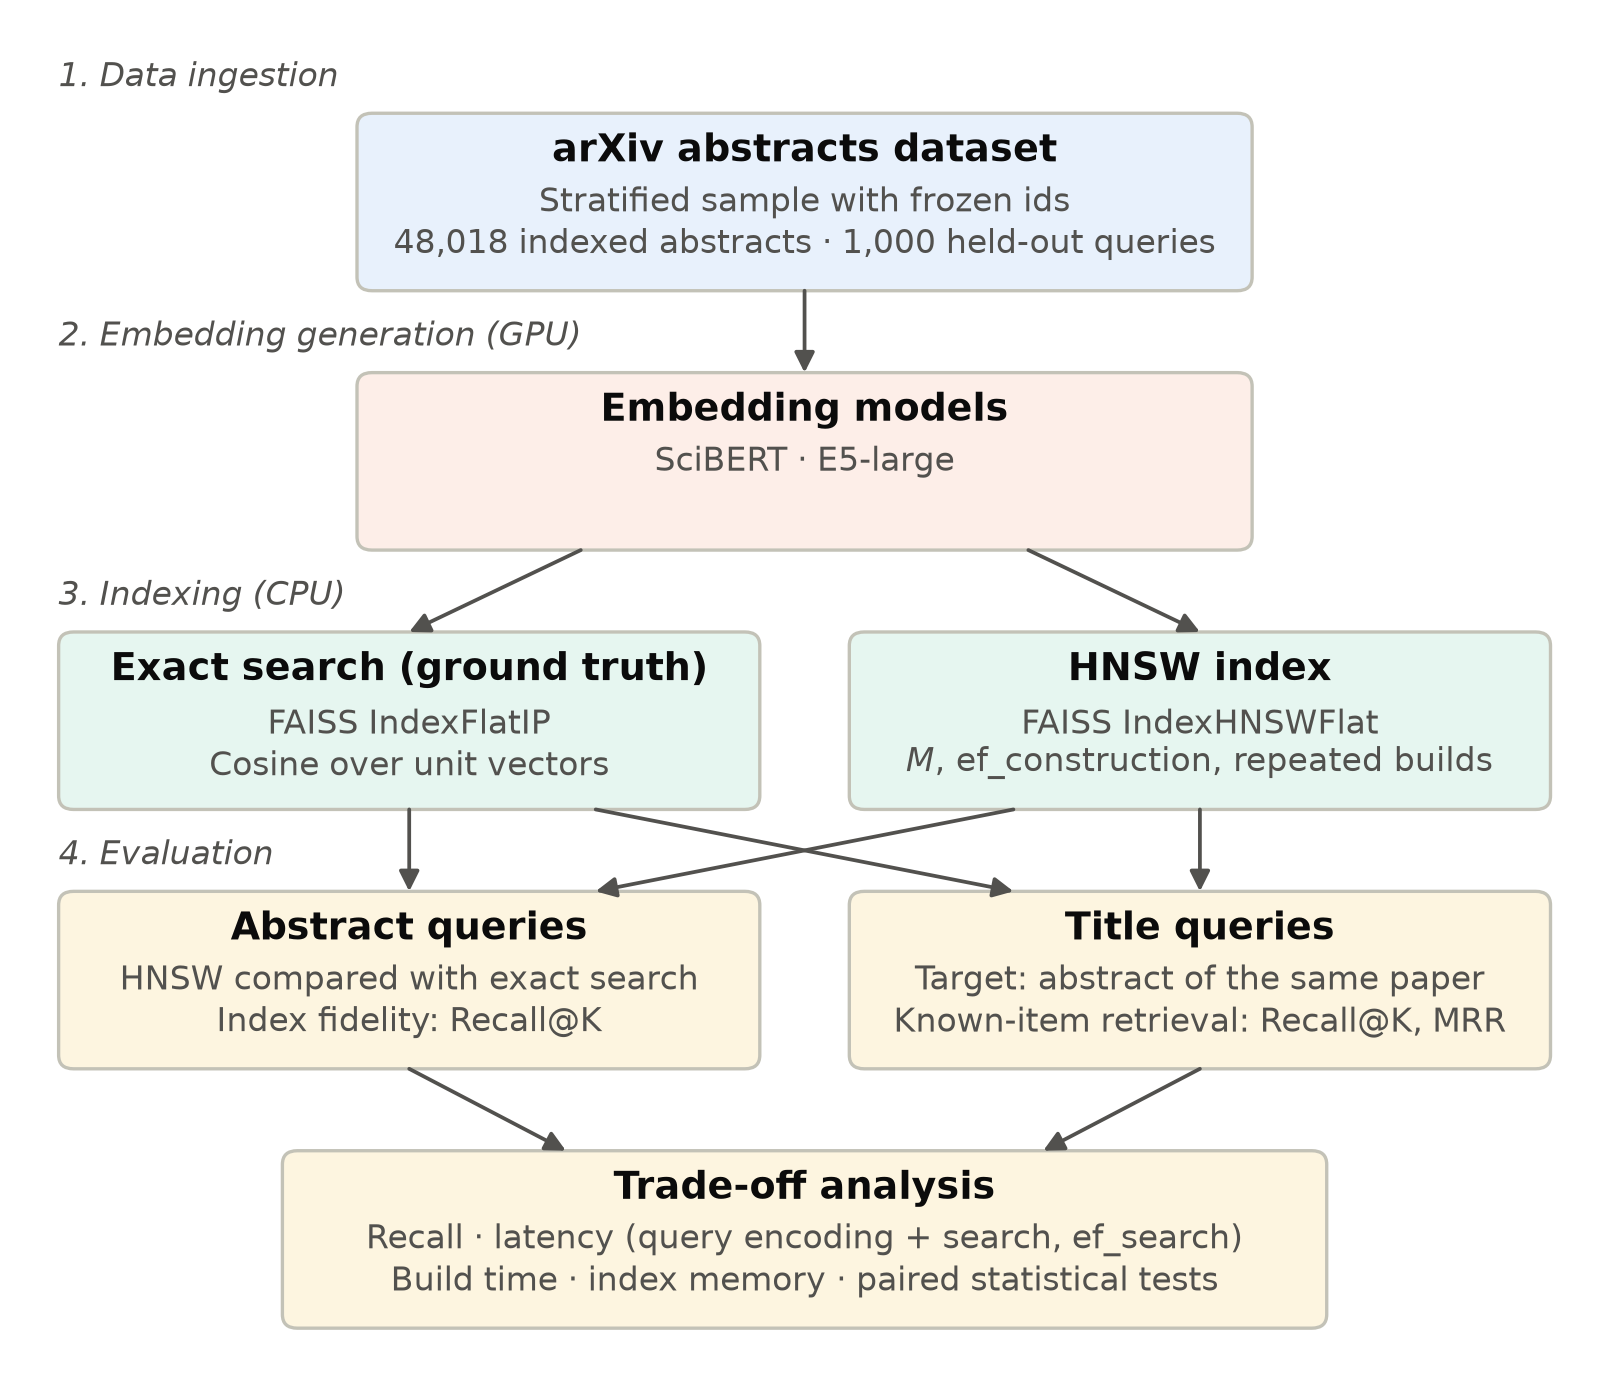
\includegraphics[width=0.68\textwidth]{Images/diagrama_bloques.png}
\caption{System block diagram}
\label{fig:diagrama}
\end{figure}

% -------------------------------------------------------
\subsection{Architecture Overview}
% -------------------------------------------------------

The computational load is distributed according to hardware requirements. The vectorization step, which is resource-intensive, is performed on an NVIDIA T4 block in Google Colab. On the other hand, the indexing and estimation steps are performed locally on the CPU, where the \texttt{FAISS} \cite{ref7} library provides sufficient performance. The interface between the two environments consists of serialized link vectors; that is, once the images are generated, the rest of the processing no longer requires the GPU. This separation reduces computational cost by limiting GPU usage to only those phases that require it and also improves the reproducibility of the experiment. A common random seed is used for the sampling and search set selection processes, thus ensuring similar results for each run

% -------------------------------------------------------
\subsection{Data Flow}
% -------------------------------------------------------

The pipeline runs in five stages: (1) ingesting and sampling the corpus \cite{ref17}; (2) vectorizing each abstract with SciBERT \cite{ref18} and E5-large \cite{ref19}; (3) computing the exact-search ground truth for each (model, metric) pair; (4) building and querying the 36 HNSW indexes over the $1\,000$ held-out queries; and (5) evaluating $\text{Recall}@K$, MRR, and latency.

% -------------------------------------------------------
\subsection{Components and Development}
% -------------------------------------------------------

Every component builds on a proven open-source library, and all paths, hyperparameters, and the random seed are kept in a single configuration to ensure reproducibility. Indexing and search rely entirely on \texttt{FAISS}; since it does not provide cosine similarity directly, we normalize the vectors and use the inner product, which is mathematically equivalent. Each run exports its metrics to a \texttt{CSV} file from which the result tables are generated automatically.

% -------------------------------------------------------
\subsection{Interactive Demonstration}
% -------------------------------------------------------

This application implements the optimal configuration for E5-large, where M is 32 and \texttt{ef\_construction} is 400. The application reuses previously generated embeddings, then reconstructs the HNSW index only once, and stores the match between each vector and the abstract text in memory. Users must enter queries in natural language; E5-large handles vectorization and searching the index. The interface returns the similarity score, ranking, and the most relevant abstract, as well as links to arXiv and the DOI. The balance between search size and latency can be adjusted in real time by modifying the \texttt{ef\_search} parameter.

Figure ~\ref{fig:demo} shows an example of the query analysis interface. The demo uses E5-large, as shown in Section ~\ref{sec:consultas-naturales}, and performs better on short natural-language queries when used in a real-world scenario. The complete code for the pipeline and the demo is available at \url{https://github.com/Lewis014/TABD}; the demo runs locally with \texttt{streamlit run code/app.py} after installing the dependencies listed in \texttt{requirements\_app.txt}.

\begin{figure}[tbp]
\centering
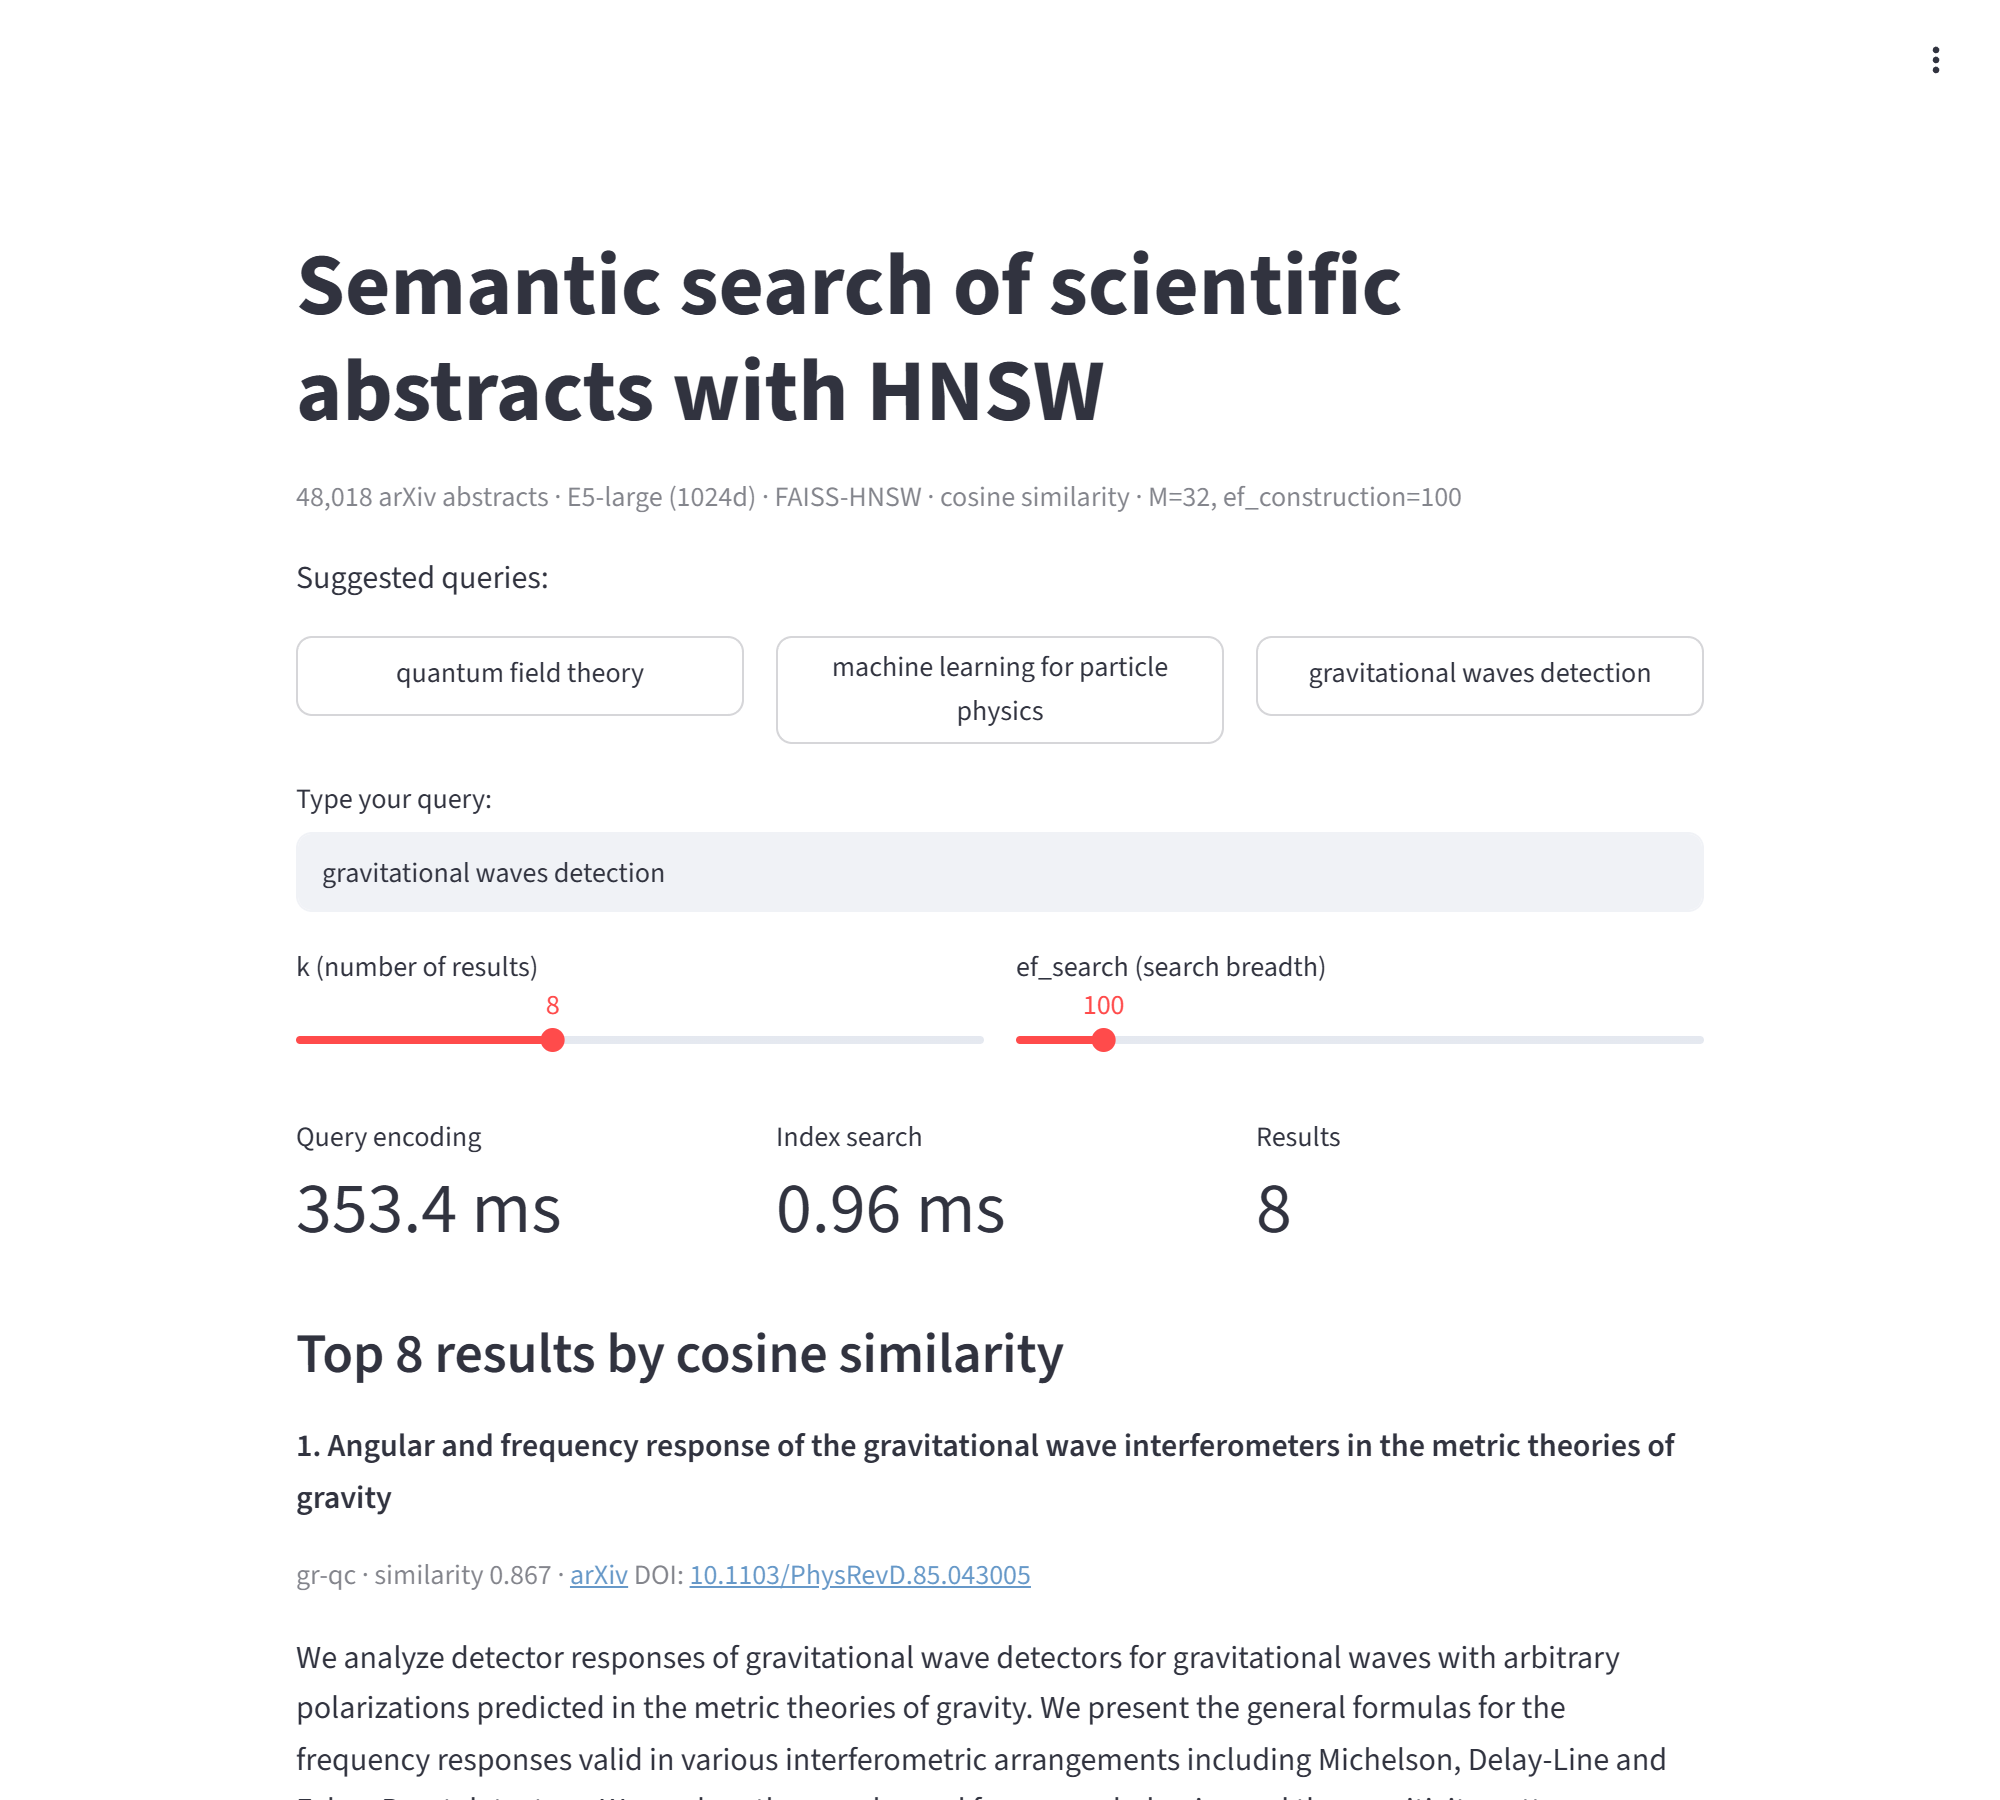
\includegraphics[width=0.95\textwidth]{Images/demo_streamlit.png}
\caption{Interactive demonstration of semantic search: the user's query
is vectorized using E5-large, and the most relevant abstracts are retrieved from the
HNSW index, with latency measured in real time.}
\label{fig:demo}
\end{figure}

% -------------------------------------------------------
\section{Results}
\label{sec:resultados}
% -------------------------------------------------------

Let's first analyze the most impressive results: all 36 configurations were successful. Even the worst-performing configuration achieved a $\text{Recall}@10$ greater than $0.94$ ($0.946$), and all configurations had response times under $1\text{~ms}$ ($0.09$–$0.70\text{~ms}$ per request). This time interval is too short to analyze, since under normal conditions the differences are minimal. However, the three factors we adjusted within this interval had a significant impact. Table~\ref{tab:resultados} shows the optimal configuration for each combination of model and metric; the complete per-configuration results (all 36 rows) are available in our public repository.\footnote{\url{https://github.com/Lewis014/TABD}}

\begin{table}[tbp]
\caption{Recall@K, MRR, and latency of the best configuration by embedding model
and similarity metric on FAISS-HNSW (49,000 documents, 1,000 queries,
\textit{ef\_search}$=50$). The best configuration is selected based on Recall@10.}
\label{tab:resultados}
\centering
\begin{tabular}{|l|l|c|c|c|c|c|c|c|}
\hline
\textbf{Model} & \textbf{Metric} & \textbf{$M$} & \textbf{\textit{ef\_c}} &
\textbf{R@1} & \textbf{R@5} & \textbf{R@10} & \textbf{MRR} & \textbf{Lat. (ms)} \\
\hline
SciBERT   & Cosine & 32 & 400 & 1.000 & 0.999 & \textbf{0.998} & 1.000 & 0.33 \\
SciBERT   & L2     & 32 & 400 & 1.000 & 0.999 & 0.998 & 1.000 & 0.25 \\
E5-large  & Cosine & 32 & 400 & 0.999 & 0.997 & 0.995 & 0.999 & 0.40 \\
E5-large  & L2     & 32 & 200 & 1.000 & 0.998 & 0.995 & 1.000 & 0.50 \\
\hline
\end{tabular}
\end{table}

Of these three parameters, the effect of $M$ is the most pronounced (Fig.~\ref{fig:recallm}). When $M = 8$, $\text{Recall}@10$ remains between $0.95$ and $0.96$; when $M$ reaches 16, $\text{Recall}@10$ slightly exceeds $0.98$; and when $M$ reaches 32, $\text{Recall}@10$ stabilizes around $0.99$. A significant increase is observed between 8 and 16: beyond 16, the index tends toward the upper limit, and therefore $\text{Recall}@10$ increases slightly. The MRR confirms this from another angle: when $M \ge 16$, the MRR stabilizes between $0.997$ and $1.000$, meaning that the first matching neighbor is almost always in the first position. 

The situation changes during the construction of the response element, which is somewhat disappointing. Increasing this parameter from 100 to 400 improves the recall at 10 ($\text{Recall}@10$) by only a few percentage points (from $0.993$ to $0.998$, and even more for the SciBERT model using the cosine transform and $M=32$), but it nearly doubles the indexing time: from approximately $15\text{~seconds}$ to $44\text{~seconds}$. The goal is not to achieve maximum precision, but to improve it. If continuous index rebuilding is required, it is more efficient to reduce this parameter than to increase it. 

Furthermore, the impact of the similarity metric is almost negligible. After vector normalization, the performance of the cosine transform and the $L_2$ distance is nearly identical: the difference in the 10-point recall rate is at most two or three thousandths of the noise. Normalization is necessary to balance the performance of the two methods; as other studies have shown, Euclidean distance modeling becomes inefficient without normalization. For this dataset, choosing one method over the other has no significant effect.

Continuing with the comparison between models, SciBERT outperforms E5-large by a small but consistent margin—0.998 versus 0.995 for Recall@10—and is also faster, at 0.33 ms per query compared to 0.40 ms for E5-large, in addition to having indexes that are built more quickly; it also occupies the region of highest accuracy and lowest latency among the 36 configurations (Fig.~\ref{fig:latencia}). The result is interesting; SciBERT works with 768-dimensional vectors and E5-large with 1,024-dimensional vectors. This means that fewer dimensions reduce the computational cost of each distance comparison, and for these abstracts, that efficiency did not come at the expense of index accuracy.

To rule out the possibility that the $0.003$ margin in $\text{Recall}@10$ is attributable to variability between queries, we subjected it to paired statistical tests. The McNemar test shows 47 queries in favor of SciBERT versus 16 in favor of E5-large among the discordant pairs, with an exact two-sided $p$-value of $0.00012$ ($p < 0.001$). The Wilcoxon signed-rank test
on $\text{Recall}@10$ per query confirms this. Therefore, SciBERT's advantage in $\text{Recall}@10$ is statistically significant and not a
random effect. On the other hand, the difference in MRR of $1.000$ versus $0.999$ is not statistically significant. Both models place the first
true neighbor in the first position almost always, so in terms of MRR they are
statistically equivalent. In summary, SciBERT outperforms E5-large
significantly in index fidelity ($\text{Recall}@10$ abstract-to-abstract), while they are equivalent in terms of MRR. However, as shown in Section~\ref{sec:consultas-naturales}, this advantage in recall does not translate to better retrieval when the query is a short natural-language phrase.

\begin{figure}[tbp]
\centering
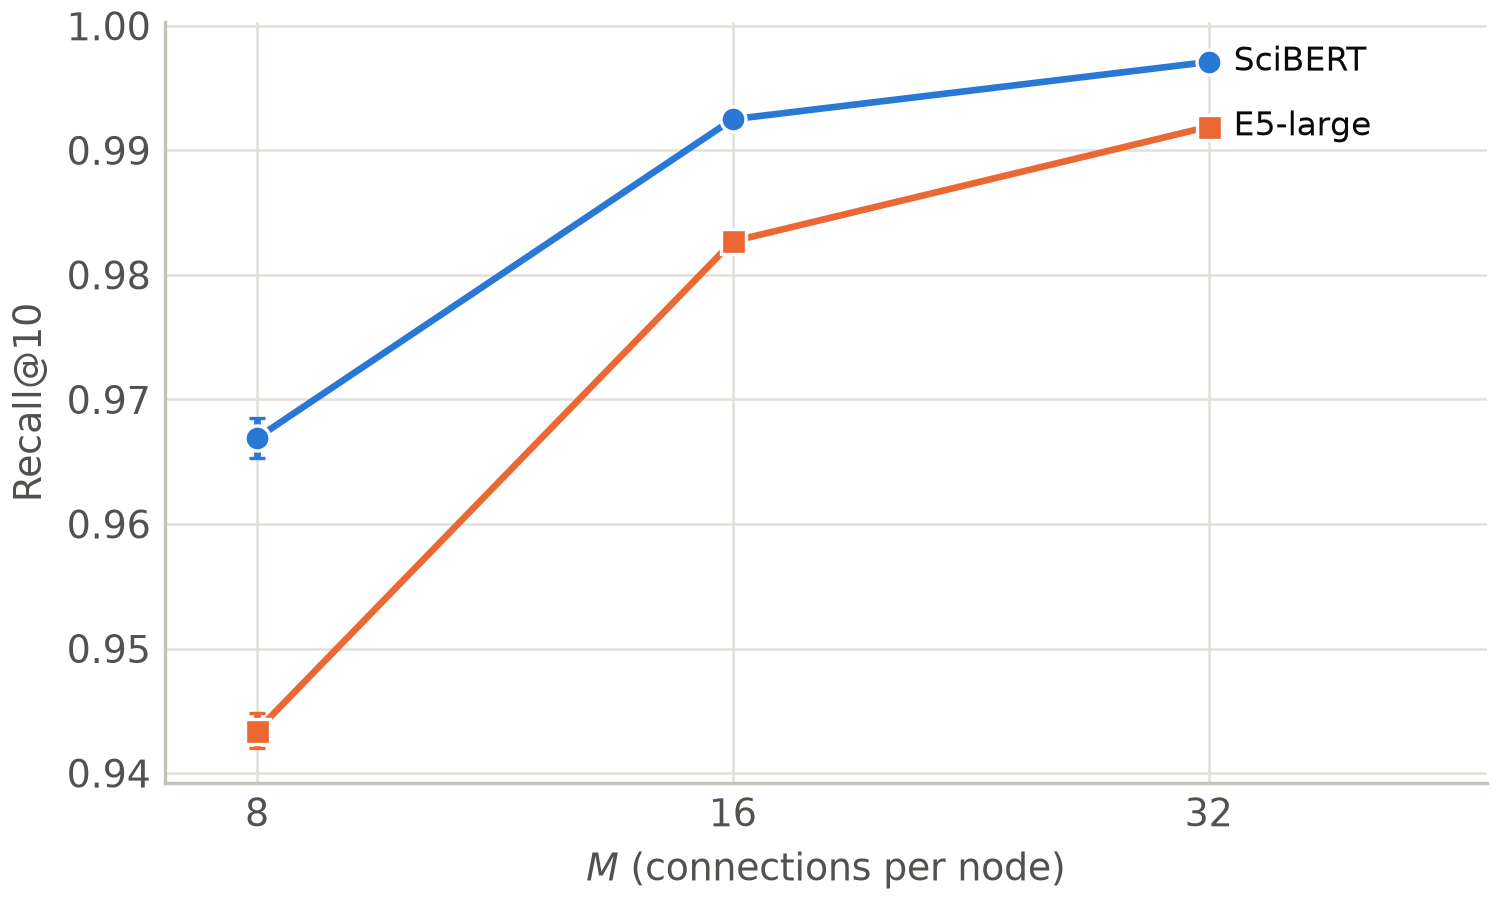
\includegraphics[width=0.72\textwidth]{Images/fig_recall_vs_m.png}
\caption{Recall@10 as a function of $M$ (with $\textit{ef\_construction}$=400) for each
combination of model and metric. The decisive jump occurs when moving from $M=8$ to $M=16$;
from 16 to 32, the improvement flattens out, and SciBERT remains above E5-large.}
\label{fig:recallm}
\end{figure}

\begin{figure}[tbp]
\centering
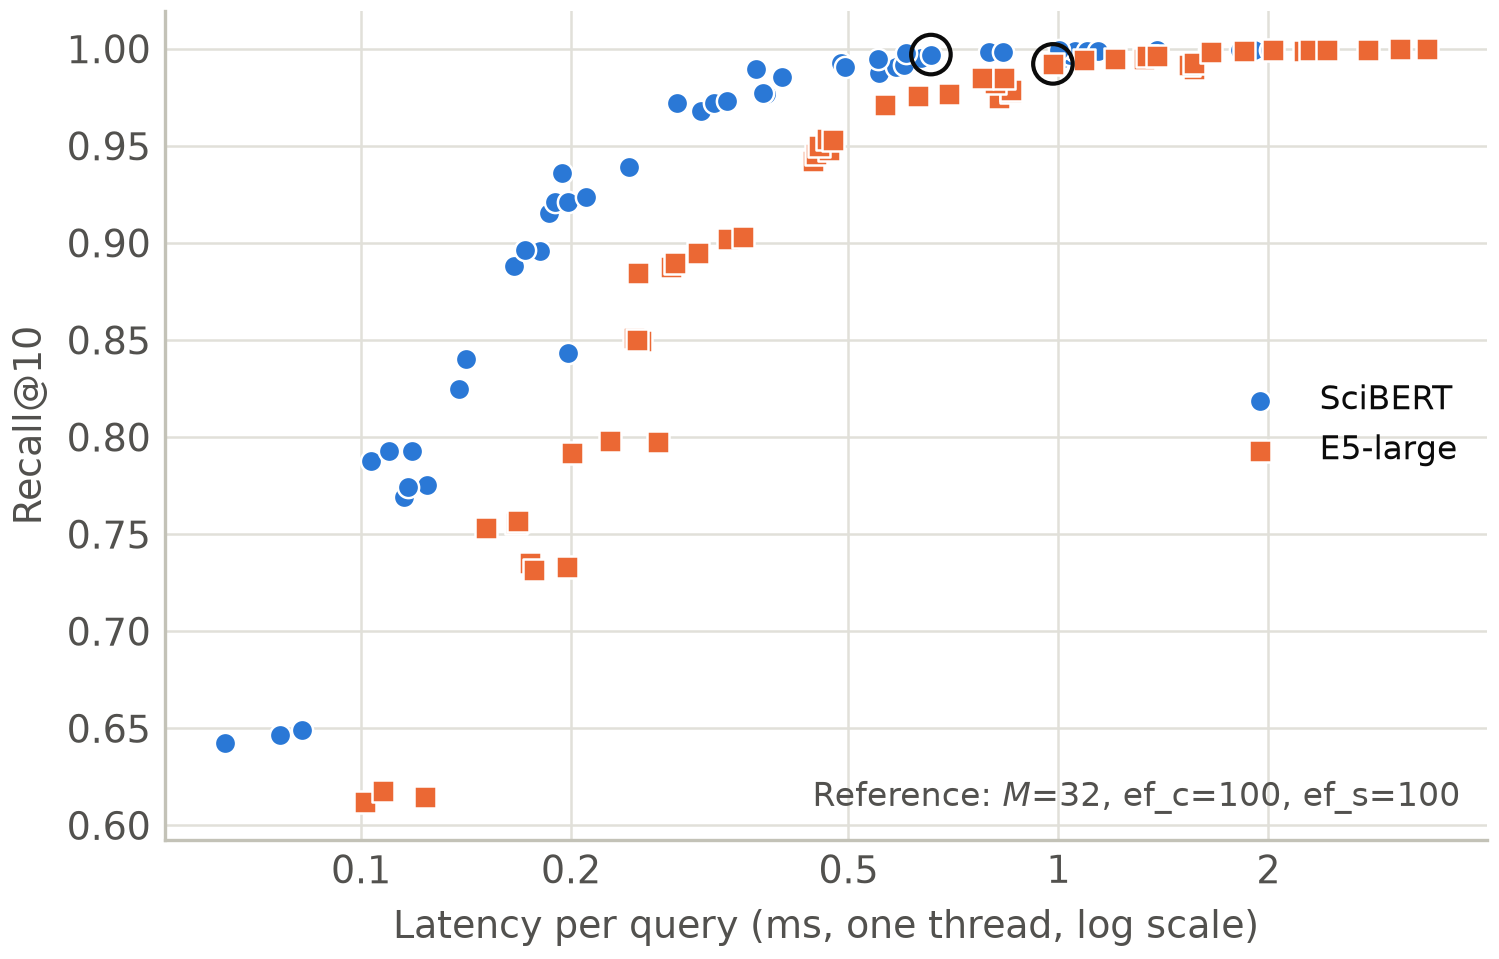
\includegraphics[width=0.72\textwidth]{Images/fig_recall_latency.png}
\caption{Trade-off between Recall@10 and latency per query for the 36
configurations. SciBERT (blue) occupies the region of highest accuracy and lowest latency,
while E5-large (red) shifts toward higher latencies.}
\label{fig:latencia}
\end{figure}

% -------------------------------------------------------
\subsection{Sensitivity of \textit{ef\_search}}
% -------------------------------------------------------

The factors mentioned above determine the index construction; however, the balance between accuracy and latency is controlled by \texttt{ef\_search}, which until now was set to 50. This value is not arbitrary; a sensitivity analysis was performed on the best configuration, which is SciBERT, cosine, $M=32$, $\textit{ef\_construction}$=400. Table~\ref{tab:efsearch} and Fig.~\ref{fig:efsearch}
summarize the results.

\begin{table}[tbp]
\caption{Sensitivity analysis of \textit{ef\_search} on the best
configuration mentioned above. The index is constructed only once, and only \textit{ef\_search} varies.}\label{tab:efsearch}
\centering
\begin{tabular}{|c|c|c|c|c|c|}
\hline
\textbf{\textit{ef\_search}} & \textbf{R@1} & \textbf{R@5} & \textbf{R@10} &
\textbf{MRR} & \textbf{Lat. (ms)} \\
\hline
10  & 0.998 & 0.985 & 0.963 & 0.998 & 0.09 \\
20  & 0.998 & 0.994 & 0.985 & 0.998 & 0.19 \\
50  & 1.000 & 0.999 & \textbf{0.998} & 1.000 & 0.32 \\
100 & 1.000 & 0.999 & 1.000 & 1.000 & 0.48 \\
200 & 1.000 & 0.999 & 1.000 & 1.000 & 0.70 \\
400 & 1.000 & 0.999 & 1.000 & 1.000 & 1.36 \\
\hline
\end{tabular}
\end{table}

The curve shows a sharp bend when \texttt{ef\_search} is 50. Below that point, $\text{Recall}@10$ drops to $0.963$, where the search breadth
barely exceeds 10 and fails to explore enough candidates. When it is greater than 100, $\text{Recall}@10$ is saturated, and the only thing that increases is latency, from $0.32$ to $1.36\text{~ms}$. 
Therefore, 50 is the optimal value in terms of
accuracy and latency; since, for this configuration, it retrieves the greatest number of true neighbors at a lower cost in terms of
latency.

\begin{figure}[tbp]
\centering
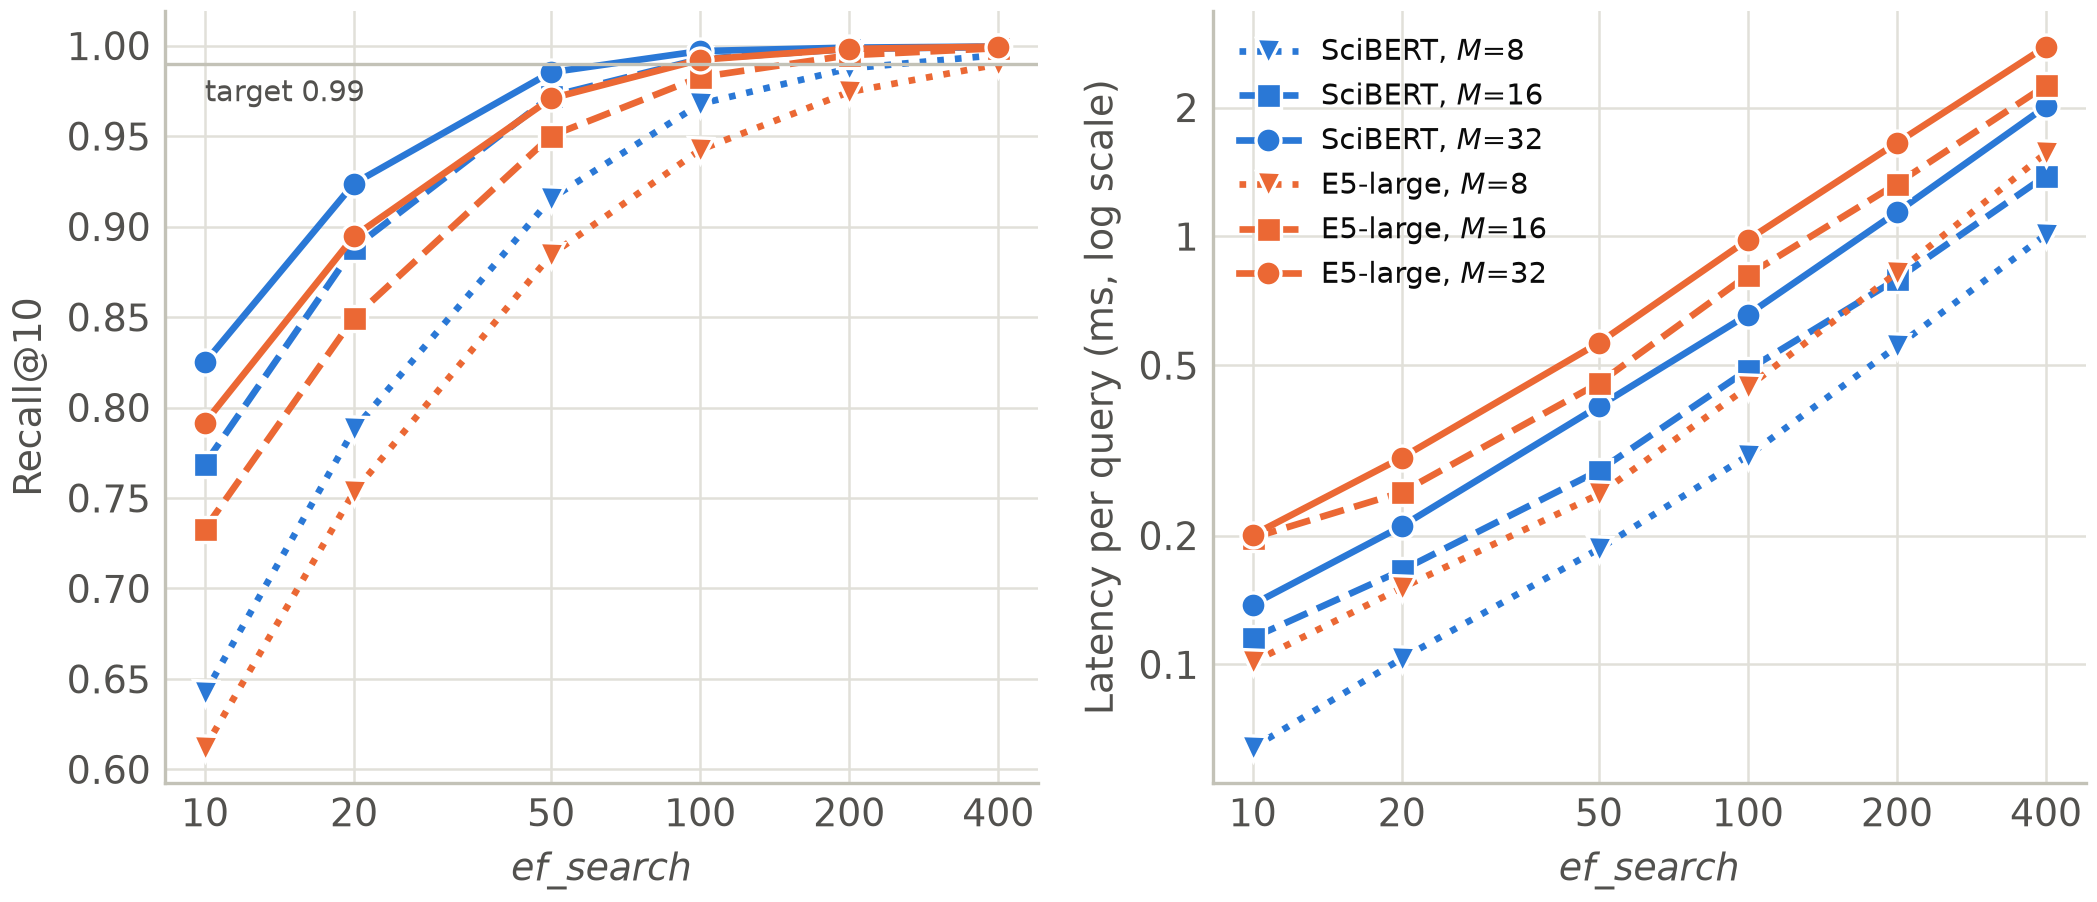
\includegraphics[width=0.72\textwidth]{Images/fig_ef_search.png}
\caption{Sensitivity of \texttt{ef\_search} regarding the best configuration, where $\text{Recall}@10$ saturates when \texttt{ef\_search} is 50, while
latency continues to increase. The value of 50 used in the study lies at the inflection point of the curve.}
\label{fig:efsearch}
\end{figure}

% -------------------------------------------------------
\subsection{Retrieval with Natural Language Queries}
\label{sec:consultas-naturales}
% -------------------------------------------------------

The previous evaluation uses full abstracts as queries, which measures the accuracy of the index; however, this is not used in the system, where the user
enters a short phrase in natural language. To address this scenario,
we designed a \textit{known-item} evaluation, in which we took a sample
of 1,000 documents from the corpus and used their titles as queries. The titles are not indexed—only the abstracts are—but the relevant document is unique, as the abstract is derived from its title. We vectorized the titles using the same method as for the
corpus and performed the search using the best configuration mentioned above. Table~\ref{tab:naturales} summarizes the results.

\begin{table}[tbp]
\caption{\textit{Known-item} retrieval: title$\rightarrow$abstract (short
natural language query) versus abstract$\rightarrow$abstract evaluation,
by model, using the best configuration (cosine, $M=32$,
\textit{ef\_construction}$=400$; 1\,000 queries).}\label{tab:naturales}
\centering
\begin{tabular}{|l|l|c|c|c|c|}
\hline
\textbf{Scenario} & \textbf{Model} & \textbf{R@1} & \textbf{R@5} &
\textbf{R@10} & \textbf{MRR} \\
\hline
Abstract$\rightarrow$abstract & SciBERT  & 1.000 & 0.999 & \textbf{0.998} & 1.000 \\
Abstract$\rightarrow$abstract & E5-large & 0.999 & 0.997 & 0.995 & 0.999 \\
\hline
Title$\rightarrow$abstract   & SciBERT  & 0.074 & 0.152 & 0.194 & 0.107 \\
Title$\rightarrow$abstract   & E5-large & 0.869 & 0.946 & \textbf{0.953} & 0.902 \\
\hline
\end{tabular}
\end{table}

The result completely reverses the comparison between models (Fig.~\ref{fig:naturales}). In the usage scenario, SciBERT plummets to a $\text{Recall}@10$ of $0.194$, while
E5-large maintains it at $0.953$. The reason is that SciBERT
is a BERT model without retrieval training, so it places each title
at an average similarity of only $0.733$ to its own abstract, which is lower than that
of other documents, whereas E5-large is trained with pairs for the asymmetric query-document matching,
which places it at $0.878$ and mostly in the top position. The superiority of
SciBERT observed earlier is limited by the index's fidelity to its
own vector space and does not translate to retrieval quality. When the query is an actual short phrase, the model to use is E5-large. This shows us that fidelity to the exact index and
retrieval utility are distinct dimensions, so the choice of model should be based on its intended use.

\begin{figure}[tbp]
\centering
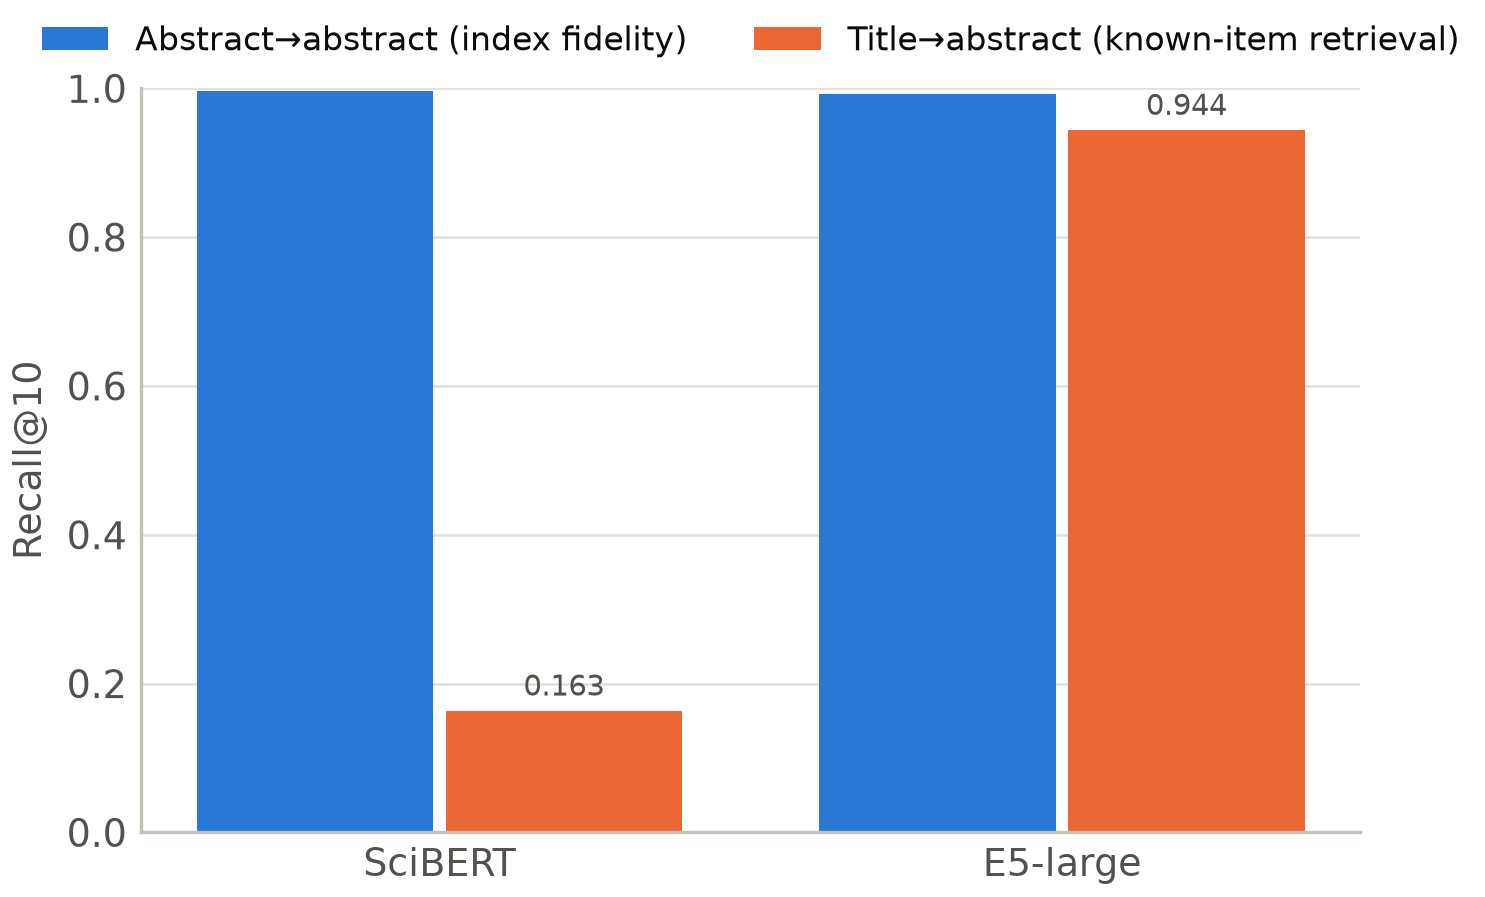
\includegraphics[width=0.72\textwidth]{Images/fig_natural_vs_fidelity.png}
\caption{Recall@10 for SciBERT and E5-large in the two scenarios. In
abstract$\rightarrow$abstract (index fidelity), both approach $1.0$ and
SciBERT has a slight edge; in title$\rightarrow$abstract (actual short
query), SciBERT drops to $0.194$ while E5-large remains at $0.953$.}
\label{fig:naturales}
\end{figure}

% -------------------------------------------------------
\subsection{Index Scalability}
\label{sec:escalabilidad}
% -------------------------------------------------------

The main experiment uses 49,000 documents, a size at which the advantage
of HNSW over exact search—whose complexity is $O(N \cdot d)$ versus
$O(\log N)$—may not be apparent. To verify this, we measured the latency per
query for both indexes on nested, reproducible subsets of the corpus,
ranging from $5\,000$ to $100\,000$ vectors (SciBERT, cosine, $M=32$,
\textit{ef\_construction}$=400$, \textit{ef\_search}$=50$).
Table~\ref{tab:escalabilidad} and Fig.~\ref{fig:escalabilidad} show the
results.

\begin{table}[tbp]
\caption{Query latency for exact search (\texttt{IndexFlatIP}) and
HNSW as a function of corpus size, with HNSW's Recall@10 compared to exact search
at the same size (1,000 queries, SciBERT, cosine).}\label{tab:escalabilidad}
\centering
\begin{tabular}{|c|c|c|c|c|}
\hline
\textbf{$N$} & \textbf{Exact (ms)} & \textbf{HNSW (ms)} &
\textbf{Speedup} & \textbf{R@10} \\
\hline
5,000   & 0.027 & 0.037 & 0.7$\times$ & 0.999 \\
10,000  & 0.057 & 0.143 & 0.4$\times$ & 0.998 \\
20,000  & 0.177 & 0.178 & 1.0$\times$ & 0.995 \\
35,000  & 0.159 & 0.262 & 0.6$\times$ & 0.992 \\
49,000  & 0.251 & 0.286 & 0.9$\times$ & 0.990 \\
75,000  & 0.366 & 0.322 & 1.1$\times$ & 0.988 \\
100\,000 & 0.505 & 0.368 & \textbf{1.4$\times$} & 0.987 \\
\hline
\end{tabular}
\end{table}

The exact search scales approximately linearly (it multiplies by 18 when going from 5,000 to 100,000 vectors), while HNSW scales sublinearly (it multiplies by 10). These different growth rates explain the crossover point around 60,000 documents: below that threshold, exact search---highly optimized using BLAS in FAISS---is just as fast or faster, and only from that point on does HNSW take the lead, with an advantage that widens to 1.4$\times$ at 100,000. This empirically confirms the limitation we had already noted: at the size of the study (49,000), the exact search is even slightly faster than HNSW, so HNSW's advantage applies to larger corpora. Recall@10 remains above 0.98 across the entire range, so HNSW maintains its accuracy as the corpus grows.

\begin{figure}[tbp]
\centering
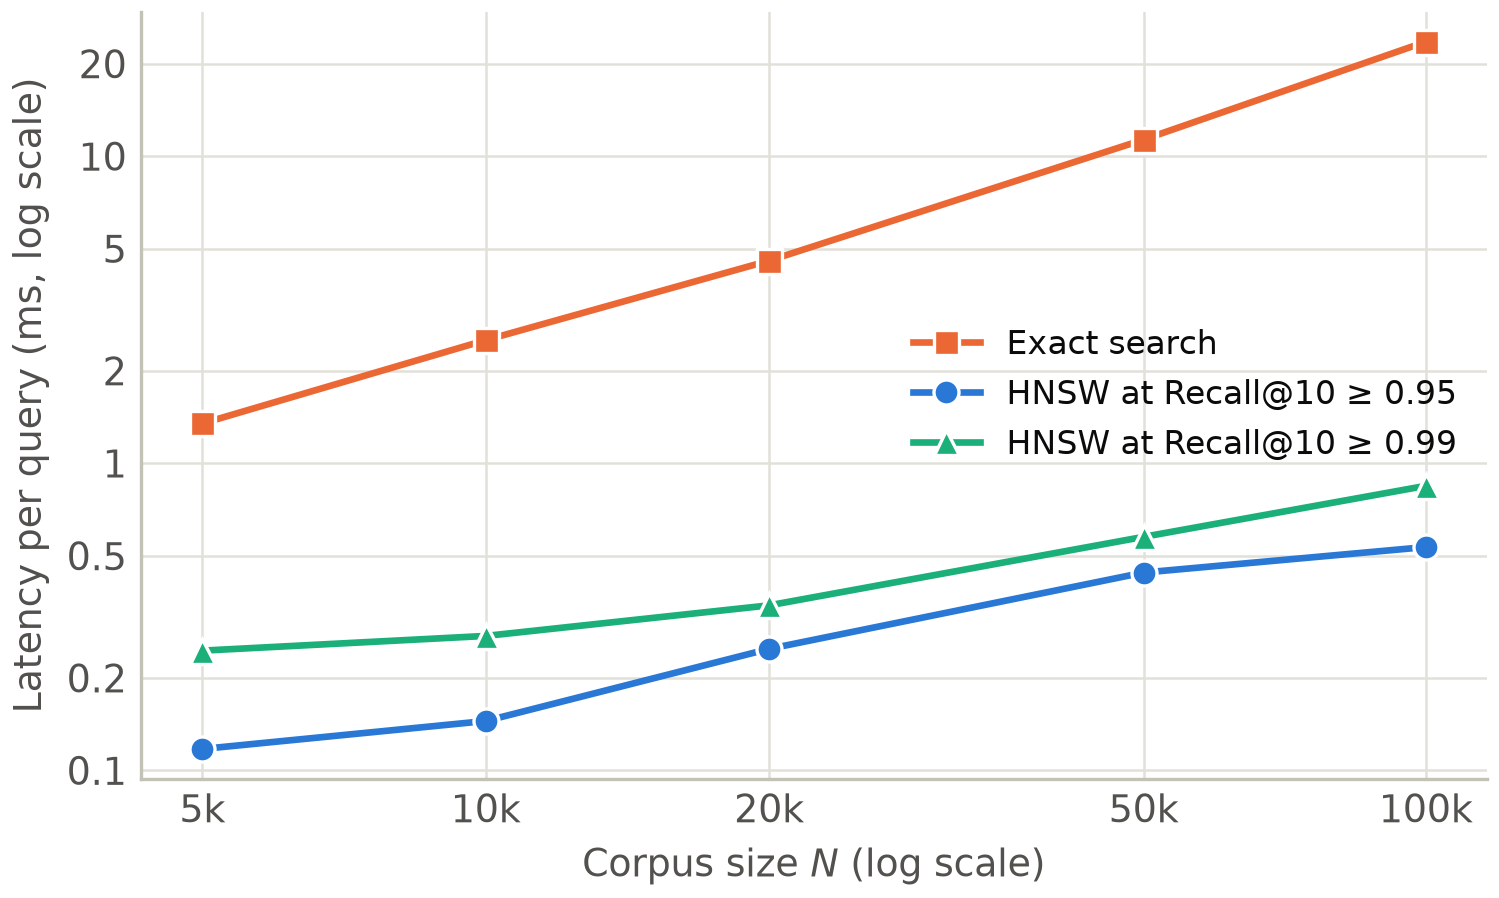
\includegraphics[width=0.72\textwidth]{Images/fig_scalability.png}
\caption{Latency per query versus corpus size. Exact search grows linearly, while HNSW grows sublinearly.}
\label{fig:escalabilidad}
\end{figure}

% -------------------------------------------------------
\section{Conclusions}
% -------------------------------------------------------

Applying the HNSW algorithm to unexplored areas constitutes a research effort 
involving dense technical terminology and multiple analytical approaches. Once 
the technical validation was completed, the evaluation using two well-defined contrasting configurations 
—employing $36$ constructs and a probabilistic analysis of extreme scenarios 
—yielded conclusive results: HNSW demonstrates high exact accuracy. 
Even under the most unfavorable configuration, it is possible to recover neighboring nodes 
in less than $1\,\text{ms}$ with $94\%$ accuracy. Its advantage in terms of speed 
lies in its ability to bound the search space without drastically sacrificing 
accuracy; a benefit that increases exponentially as the size 
of the corpus or database grows (Section 5.3). 

The behavior of this algorithm is extensively documented in the scientific literature. 
Among its many parameters, $M$ stands out as the most critical, since it determines the 
optimal balance between accuracy and computational cost. Meanwhile, although the parameter 
\textit{ef\_construction} has a minor impact on its own, it offers significant 
leeway for configuration tuning. Consistent results were obtained by 
normalizing the magnitude of the vectors. In particular, the SciBERT model provides 
a fast and accurate search process; however, in real production environments 
this advantage may be diminished when handling short queries formulated in natural language. 
Therefore, the selection of the optimal model will depend strictly on the specific use case. 

Based on these findings, fundamental heuristic recommendations are derived for the 
implementation of similar algorithms in practical settings: if the scenario does not require 
extreme precision, a robust strategy is to select a medium or 
high value for $M$, while keeping \textit{ef\_construction} within an intermediate range to 
efficiently process natural language queries. In short, this paper establishes a 
comprehensive methodological framework that allows for the configuration and deployment of the 
end-to-end search system without requiring additional parameterizations.

% -------------------------------------------------------
\section{Discussion}
% -------------------------------------------------------

It is important not to be misled by absolute numbers. A $\text{Recall}@10$ of $0.998$ measures how faithfully HNSW approximates an exact search over the \emph{same} vector space, not the relevance of the results to a user: the ground truth of Section~3.4 compares HNSW against itself, without human relevance judgments. It is the embedding model, not the index, that ultimately determines relevance. Our natural-language evaluation (Section~\ref{sec:consultas-naturales}) confirms this empirically: keeping the index structure fixed and replacing SciBERT with E5-large raises $\text{Recall}@10$ from $0.19$ to $0.95$.

Our study has three main limitations. First, the \textit{known-item} evaluation mitigates but does not replace an external validation with human relevance judgments or an established benchmark (BEIR, TREC-COVID, NFCorpus, SciFact). Second, \texttt{ef\_search} was fixed at 50 and its sensitivity analyzed only for $M=32$; the full cross-interaction between \texttt{ef\_search}, $M$, and \texttt{ef\_construction} was not explored. Third, the corpus ($49\,000$ documents) is modest: our scalability analysis (Section~\ref{sec:escalabilidad}) shows that HNSW's speed advantage over exact search only emerges beyond about $60\,000$ documents, and confirming this trend on millions of documents remains pending.

To the best of our knowledge, no previous work has measured these trade-offs on scientific abstracts. Our contribution is to compare, directly and on the same corpus, a domain-specific embedding against a general-purpose retrieval model, showing that their ranking reverses depending on whether index fidelity or real-query retrieval is measured. Future work includes evaluating indexing under heavier workloads and larger corpora, testing multilingual or other domain-specific models, and incorporating human relevance judgments to validate semantic relevance.


% -------------------------------------------------------
% References — listed in the order of their first appearance in the text
% -------------------------------------------------------

\begin{thebibliography}{19}

\bibitem{ref1}
arXiv, ``arXiv Submission Statistics,'' Cornell University.\\
\url{https://arxiv.org/stats/monthly_submissions}, last accessed May 2026.

\bibitem{ref2}
U.S. National Library of Medicine, ``MEDLINE/PubMed Production Statistics.''\\
\url{https://www.nlm.nih.gov/bsd/medline_pubmed_production_stats.html},
last accessed May 2026.

\bibitem{ref3}
N. Reimers and I. Gurevych, ``Sentence-BERT: Sentence Embeddings Using Siamese
BERT-Networks,'' in \textit{Proc. 2019 Conf. Empirical Methods in Natural Language
Processing (EMNLP-IJCNLP)}, 2019, pp. 3982--3992.\\
\url{https://doi.org/10.18653/v1/D19-1410}

\bibitem{ref4}
S. Mathur and A. Chhabra, ``Vector Search Algorithms: A Brief Survey,'' in
\textit{Proc. Int. Conf. on Emerging Technologies}, IEEE, 2024.

\bibitem{ref5}
Y. A. Malkov and D. A. Yashunin, ``Efficient and Robust Approximate Nearest
Neighbor Search Using Hierarchical Navigable Small World Graphs,'' \textit{IEEE
Trans. Pattern Anal. Mach. Intell.}, vol. 42, no. 4, pp. 824--836, 2020.\\
\url{https://doi.org/10.1109/TPAMI.2018.2889473}

\bibitem{ref6}
D. J. Watts and S. H. Strogatz, ``Collective Dynamics of `Small-World' Networks,''
\textit{Nature}, vol. 393, no. 6684, pp. 440--442, 1998.\\
\url{https://doi.org/10.1038/30918}

\bibitem{ref7}
J. Johnson, M. Douze, and H. J\'egou, ``Billion-Scale Similarity Search with
GPUs,'' \textit{IEEE Trans. Big Data}, vol. 7, no. 3, pp. 535--547, 2021.\\
\url{https://doi.org/10.1109/TBDATA.2019.2921572}

\bibitem{ref8}
J. Wang \textit{et al.}, ``Milvus: A Purpose-Built Vector Data Management System,''
in \textit{Proc. ACM Int. Conf. Management of Data (SIGMOD)}, 2021,
pp. 2614--2627.\\
\url{https://doi.org/10.1145/3448016.3457550}

\bibitem{ref9}
F. Zhao, D. Liu, and Y. Wang, ``Hierarchical HNSW Index Construction Method Based
on Maximum Distance Constraint,'' in \textit{Proc. 5th Int. Conf. Digital Society
and Intelligent Systems (DSInS)}, IEEE, 2025.

\bibitem{ref10}
P. Lewis \textit{et al.}, ``Retrieval-Augmented Generation for Knowledge-Intensive
NLP Tasks,'' in \textit{Advances in Neural Information Processing Systems
(NeurIPS)}, vol. 33, 2020, pp. 9459--9474.\\
\url{https://doi.org/10.48550/arXiv.2005.11401}

\bibitem{ref11}
H. Elkiran and J. Rasheed, ``Systematic Evaluation of Similarity Metrics for
Retrieval, Reranking, and Completion in Retrieval Augmented Generation Systems,''
in \textit{Proc. IEEE Int. Conf. Emerging Trends in Engineering and Computing
(ETE-COM)}, IEEE, 2025.

\bibitem{ref12}
P. Rajpurkar, J. Zhang, K. Lopyrev, and P. Liang, ``SQuAD: 100,000+ Questions for
Machine Comprehension of Text,'' in \textit{Proc. 2016 Conf. Empirical Methods in
Natural Language Processing (EMNLP)}, 2016, pp. 2383--2392.\\
\url{https://doi.org/10.48550/arXiv.1606.05250}

\bibitem{ref13}
M. Iwasaki and D. Miyazaki, ``Optimization of Indexing Based on k-Nearest Neighbor
Graph for Proximity Search in High-Dimensional Data,'' arXiv preprint
arXiv:1810.07355, 2018.\\
\url{https://doi.org/10.48550/arXiv.1810.07355}

\bibitem{ref14}
X. Zhao, Y. Tian, K. Huang, B. Zheng, and X. Zhou, ``Towards Efficient Index
Construction and Approximate Nearest Neighbor Search in High-Dimensional Spaces,''
\textit{Proc. VLDB Endowment}, vol. 16, no. 8, pp. 1979--1991, 2023.\\
\url{https://doi.org/10.14778/3594512.3594527}

\bibitem{ref15}
H. J\'egou, M. Douze, and C. Schmid, ``Product Quantization for Nearest Neighbor
Search,'' \textit{IEEE Trans. Pattern Anal. Mach. Intell.}, vol. 33, no. 1,
pp. 117--128, 2011.\\
\url{https://doi.org/10.1109/TPAMI.2010.57}

\bibitem{ref16}
C. D. Manning, P. Raghavan, and H. Sch\"utze, \textit{Introduction to Information
Retrieval}. Cambridge University Press, 2008.

\bibitem{ref17}
C. B. Clement, M. Bierbaum, K. P. O'Keeffe, and A. A. Alemi, ``On the Use of ArXiv
as a Dataset,'' arXiv preprint arXiv:1905.00075, 2019.\\
\url{https://doi.org/10.48550/arXiv.1905.00075}

\bibitem{ref18}
I. Beltagy, K. Lo, and A. Cohan, ``SciBERT: A Pretrained Language Model for
Scientific Text,'' in \textit{Proc. 2019 Conf. Empirical Methods in Natural
Language Processing (EMNLP-IJCNLP)}, 2019, pp. 3615--3620.\\
\url{https://doi.org/10.18653/v1/D19-1371}

\bibitem{ref19}
L. Wang \textit{et al.}, ``Text Embeddings by Weakly-Supervised Contrastive
Pre-training,'' arXiv preprint arXiv:2212.03533, 2022.\\
\url{https://doi.org/10.48550/arXiv.2212.03533}

\end{thebibliography}

\end{document}
